
\documentclass[a0,landscape]{a0poster}

\usepackage{multicol} %
\columnsep=100pt 
\columnseprule=3pt 

\usepackage{listings}
\usepackage[usenames,dvipsnames]{color}

\usepackage{times} % Use the times font

\usepackage{graphicx} 
\graphicspath{{figures/}}
\usepackage{booktabs} % Top and bottom rules for table
\usepackage[font=small, labelfont=bf]{caption} % Required for specifying captions to tables and figures
\usepackage{amsfonts, amsmath, amsthm, amssymb} % For math fonts, symbols and environments

\def\graphspacing{\vspace{.5cm}}
\newcommand{\highlight}[1]{{\color{Fuchsia} \textit{#1}}}
\newcommand{\capcolor}[1]{{\color{Black} #1}}
\newcommand{\var}[1]{{\small \textit{#1}}}

\begin{document}

%%%%%%%%%%%%%%%%%%%%%%%%%%%%%%%%%%%%%%%%%%%%%%%%%%%%%%%%%%%%%%%%%%%%%%%%%%%%%%%%%%%%%%%%%%%%%%%%%%
%%%%%%%%%%%%%%%%%%%%%%%%%%%%%%%%%%%%% Header %%%%%%%%%%%%%%%%%%%%%%%%%%%%%%%%%%%%%%%%%%%%%%%%%%%%%
%%%%%%%%%%%%%%%%%%%%%%%%%%%%%%%%%%%%%%%%%%%%%%%%%%%%%%%%%%%%%%%%%%%%%%%%%%%%%%%%%%%%%%%%%%%%%%%%%%
\begin{minipage}[b]{0.2\linewidth}
\centering

\includegraphics[width=.75\linewidth]{logos/mcmaster_logo}  
\end{minipage}
%
\begin{minipage}[b]{0.6\linewidth}
\centering
\veryHuge \color{Blue} \textbf{Formal Verification of IEC 61131-3 Function Blocks} \color{Black}  \\ [1cm]
\huge \textbf{Linna Pang, Chen-Wei Wang, Mark Lawford, and Alan Wassyng} \\ 
\huge McMaster Centre for Software Certification, McMaster University \\
\LARGE \texttt{\{~pangl, wangcw, lawford, wassyng~\}@mcmaster.ca}
\end{minipage}
%
\begin{minipage}[b]{0.2\linewidth}
\centering

\includegraphics[width=.45\linewidth]{logos/McScert_logo4}
\end{minipage}

\vspace{1cm} 

\begin{multicols}{4} 
	
	\normalsize
	
% \large

%%%%%%%%%%%%%%%%%%%%%%%%%%%%%%%%%%%%%%%%%%%%%%%%%%%%%%%%%%%%%%%%%%%%%%%%%%%%%%%%%%%%%%%%%%%%%%%%%%
%%%%%%%%%%%%%%%%%%%%%%%%%%%%%%%%%%%%% Abstract %%%%%%%%%%%%%%%%%%%%%%%%%%%%%%%%%%%%%%%%%%%%%%%%%%%
%%%%%%%%%%%%%%%%%%%%%%%%%%%%%%%%%%%%%%%%%%%%%%%%%%%%%%%%%%%%%%%%%%%%%%%%%%%%%%%%%%%%%%%%%%%%%%%%%%
{\color{Blue} % Navy color for the abstract

\begin{abstract}
\noindent
\begin{itemize}
\item Many industrial control systems use programmable logic controllers (PLCs) since they provide a highly reliable, off-the-shelf hardware platform. 
\item On the programming side, function blocks (FBs) are reusable components provided by the PLC supplier that can be combined to implement the required system behaviour. 
\item A higher quality system may be realized if the FBs are pre-certified to be compliant with an international standard such as IEC~61131-3. 
\item We present an approach: 
\begin{itemize}
\item to creating complete and unambiguous FB requirements using tabular expressions
\item to verifying the consistency and correctness of FB implementations in the PVS proof environment
\end{itemize}
\item We apply our approach to the IEC~61131-3 standard, by examining the entire library of FBs and their supplied implementations described in structured text (ST) and function block diagrams (FBDs). 
\item Our approach identified issues in the standard, including: a) ambiguous behavioural descriptions; b) missing assumptions; c) mismatched types of related variables; and d) erroneous implementations. 
\item We also provide resolutions to the identified issues.
\end{itemize}

\end{abstract}}

%%%%%%%%%%%%%%%%%%%%%%%%%%%%%%%%%%%%%%%%%%%%%%%%%%%%%%%%%%%%%%%%%%%%%%%%%%%%%%%%%%%%%%%%%%%%%%%%%%
%%%%%%%%%%%%%%%%%%%%%%%%%%%%%%%%%%%%% Background %%%%%%%%%%%%%%%%%%%%%%%%%%%%%%%%%%%%%%%%%%%%%%%%%
%%%%%%%%%%%%%%%%%%%%%%%%%%%%%%%%%%%%%%%%%%%%%%%%%%%%%%%%%%%%%%%%%%%%%%%%%%%%%%%%%%%%%%%%%%%%%%%%%%

{\color{Blue} \subsection*{Background}}

\begin{itemize}
	
\item \highlight{IEC~61131-3}~\cite{IEC:2003:IEP} is a standard with over 20 years of use on critical systems running on programmable logic controllers (PLCs). 	
\item \highlight{Function blocks (FBs)} are basic design units that implement the behaviour of a  PLC, where each FB is a reusable component for building new, more sophisticated components or systems. 
\item A function block typically has a natural language description of the block behaviour, accompanied by a detailed implementation in the \highlight{structured text (ST)} or \highlight{function block diagrams (FBD)} description, or in some cases both.

\item \highlight{Tabular expressions} (a.\,k.\,a.\ function tables or tables) are a promising way for documenting system requirement that has proven to be both practical and effective in industry~\cite{Wassyng2003}.
\item \highlight{Prototype Verification System (PVS)}~\cite{Owre1992} is a general-purpose theorem prover that provides an integrated environment with mechanized support for: 
\begin{itemize}
\item writing \highlight{specifications} using tabular expressions and (higher-order) predicates 
\item conducting (interactively) \highlight{proofs} that implementations satisfy the tabular requirements using sequent-style deductions
\end{itemize}
\end{itemize}

%%%%%%%%%%%%%%%%%%%%%%%%%%%%%%%%%%%%%%%%%%%%%%%%%%%%%%%%%%%%%%%%%%%%%%%%%%%%%%%%%%%%%%%%%%%%%%%%%%
%%%%%%%%%%%%%%%%%%%%%%%%%%%%%%%%%%%%% Motivation %%%%%%%%%%%%%%%%%%%%%%%%%%%%%%%%%%%%%%%%%%%%%%%%%
%%%%%%%%%%%%%%%%%%%%%%%%%%%%%%%%%%%%%%%%%%%%%%%%%%%%%%%%%%%%%%%%%%%%%%%%%%%%%%%%%%%%%%%%%%%%%%%%%%

{\color{Blue} \subsection*{Motivation}}

\begin{itemize}
\item IEC~61131-3 uses FB descriptions that are too close to the level of hardware implementations, making it difficult to argue about the behavioural correctness of FBs.
\item The search for higher quality may be realized if the FBs are pre-certified with respect to IEC~61131-3. 
\item Two acceptance criteria of mission- or safety-critical systems:
\begin{itemize}
\item The system requirements are precise and complete.
\item The system implementation exhibits behaviour that conforms to these requirements.
\end{itemize}
\item Formal descriptions, e.g., tabular expressions, prevent FB tool vendors and users from interpreting the expected behaviours differently. 
\item Formal descriptions are amenable to mechanized support, e.g., PVS, for verifying the conformance of candidate implementations to the high-level, input-output requirements.
\end{itemize}

%%%%%%%%%%%%%%%%%%%%%%%%%%%%%%%%%%%%%%%%%%%%%%%%%%%%%%%%%%%%%%%%%%%%%%%%%%%%%%%%%%%%%%%%%%%%%%%%%%
%%%%%%%%%%%%%%%%%%%%%%%%%%%%%%%%%%%% Contributions %%%%%%%%%%%%%%%%%%%%%%%%%%%%%%%%%%%%%%%%%%%%%%%
%%%%%%%%%%%%%%%%%%%%%%%%%%%%%%%%%%%%%%%%%%%%%%%%%%%%%%%%%%%%%%%%%%%%%%%%%%%%%%%%%%%%%%%%%%%%%%%%%%

{ \color{BrickRed}
\subsection*{Contributions}

\begin{enumerate}
\item A practical methodology for formally verifying function blocks compliant with IEC~61131-3.
\item Identification of issues in IEC~61131-3 example function blocks, consisting of: 
\begin{enumerate}
\item ambiguous behavioural descriptions (e.g., \var{PULSE} timer)
\item missing assumptions (e.g., \var{HYSTERESIS} and \var{LIMITS\_ALARM})
\item mismatched types of related variables (e.g., \var{PID} and \var{AVERAGE})
\item erroneous implementations (e.g., \var{STACK\_INT})
\end{enumerate}
\item Suggested resolutions of all identified issues.
\end{enumerate}
}

%%%%%%%%%%%%%%%%%%%%%%%%%%%%%%%%%%%%%%%%%%%%%%%%%%%%%%%%%%%%%%%%%%%%%%%%%%%%%%%%%%%%%%%%%%%%%%%%%%
%%%%%%%%%%%%%%%%%%%%%%%%%%%%%%%%%%%%% Methodology %%%%%%%%%%%%%%%%%%%%%%%%%%%%%%%%%%%%%%%%%%%%%%%%
%%%%%%%%%%%%%%%%%%%%%%%%%%%%%%%%%%%%%%%%%%%%%%%%%%%%%%%%%%%%%%%%%%%%%%%%%%%%%%%%%%%%%%%%%%%%%%%%%%

{\color{Blue} \subsection*{Methodology}}

\begin{center}\graphspacing
\centering
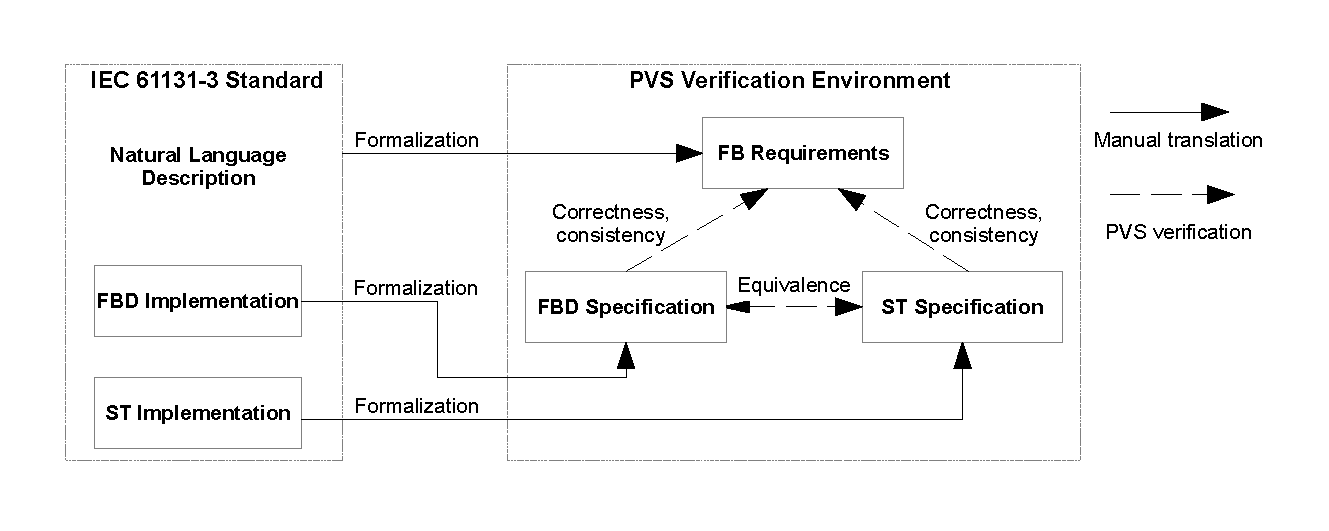
\includegraphics[width=\linewidth]{figures/methodology}
% \captionof{figure}{\capcolor{Framework of Formalization and Verification}} 
\label{fig:framework}
\end{center}\graphspacing

\begin{enumerate} 
\item Create a tabular expression requirements specification in PVS for each FB.
\item Formalize both ST and FBD implementations in PVS as higher-order predicates modelled as timed trajectories. 
\item Prove functional equivalence using PVS of the ST and FBD implementations when both are supplied in the standard. 
\item Use PVS to prove {\color{BrickRed} \textit{consistency}} and {\color{BrickRed} \textit{correctness}} of each implementation with respect to its requirements specification.
\end{enumerate}


%%%%%%%%%%%%%%%%%%%%%%%%%%%%%%%%%%%%%%%%%%%%%%%%%%%%%%%%%%%%%%%%%%%%%%%%%%%%%%%%%%%%%%%%%%%%%%%%%%
%%%%%%%%%%%%%%%%%%%%%%%%%%%%%%%%%%%%% Hysteresis %%%%%%%%%%%%%%%%%%%%%%%%%%%%%%%%%%%%%%%%%%%%%%%%%
%%%%%%%%%%%%%%%%%%%%%%%%%%%%%%%%%%%%%%%%%%%%%%%%%%%%%%%%%%%%%%%%%%%%%%%%%%%%%%%%%%%%%%%%%%%%%%%%%%

{\color{Blue} \subsection*{Example of Basic FBs: Hysteresis}}

\noindent Based on the input-output declaration and ST implementation, as suppled by IEC~61131-3~\cite{IEC:2003:IEP}:

% HYSTERESIS: declaration and ST implementation
\begin{center}\graphspacing
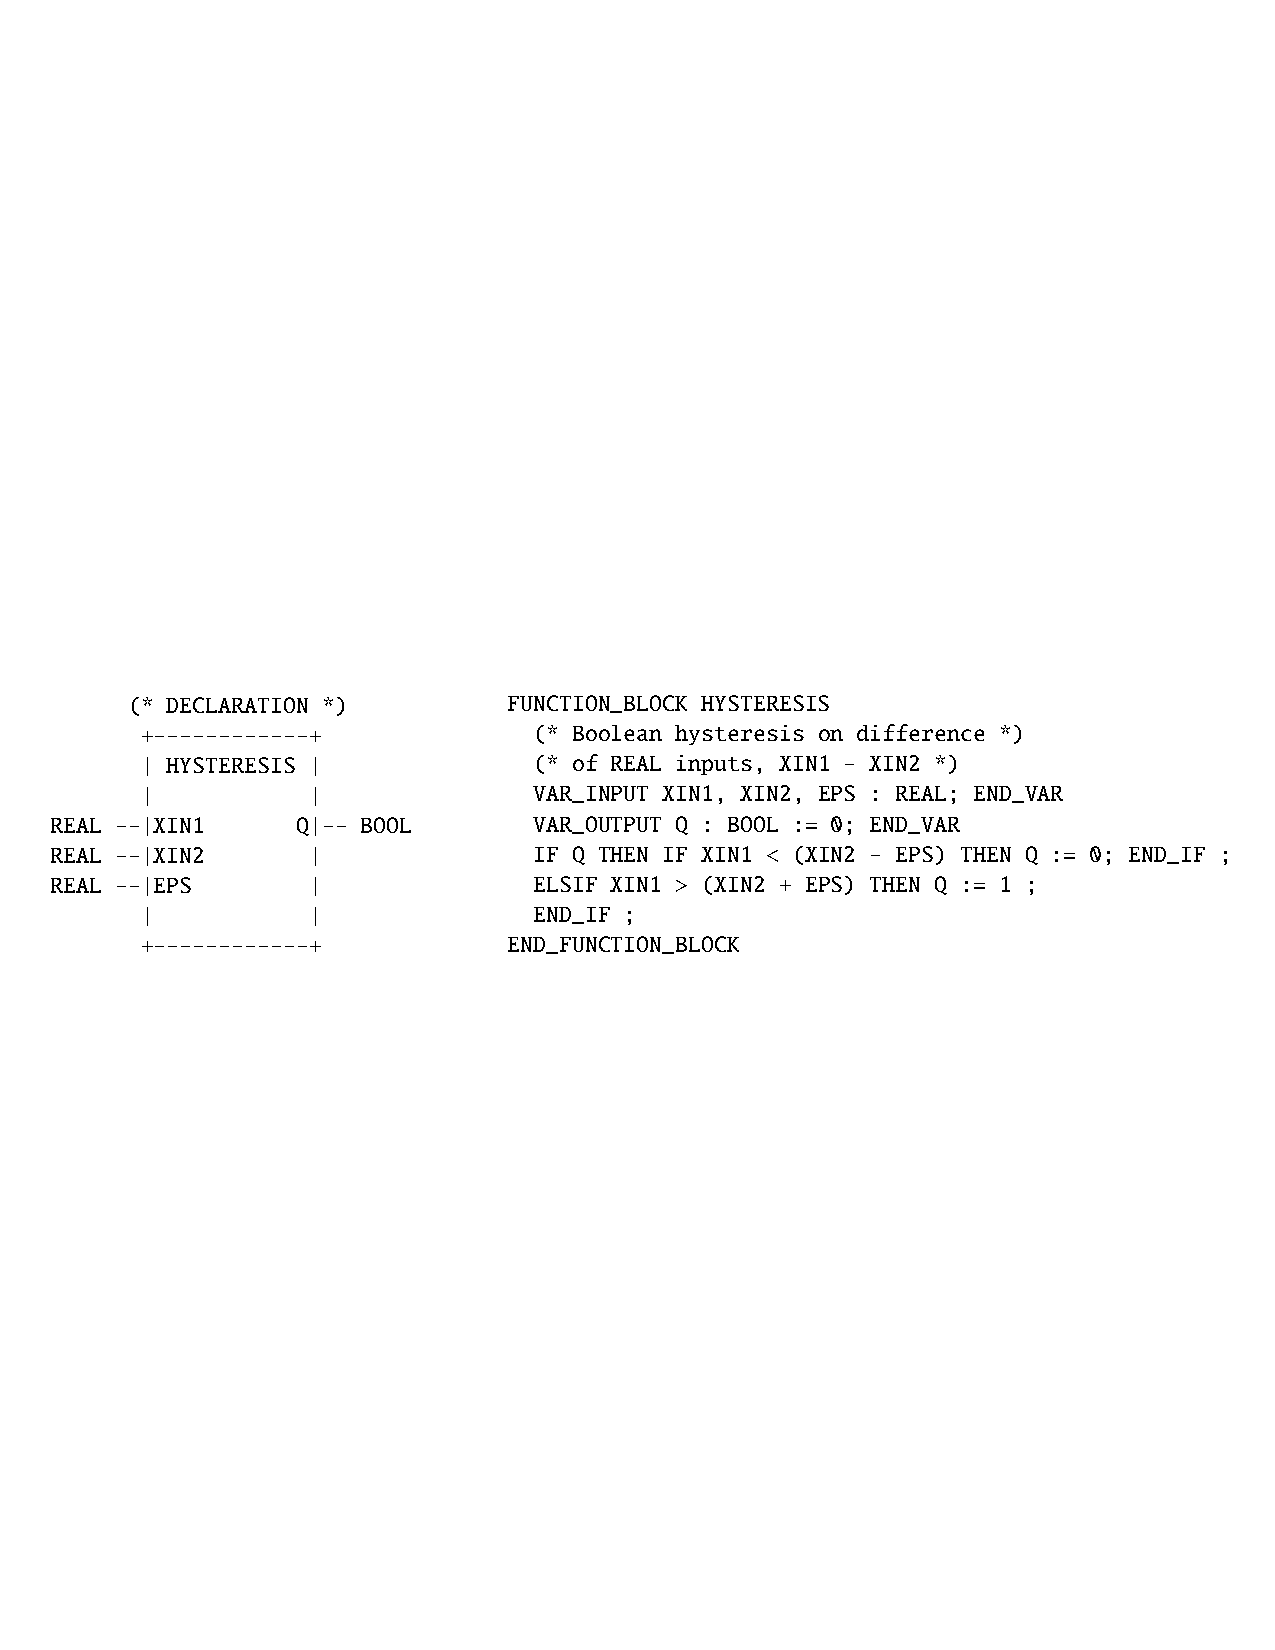
\includegraphics[width=\linewidth]{figures/hysteresis/hysteresis_decl}
% \captionof{figure}{\capcolor{Hysteresis: Declaration and ST Implementation~\cite{IEC:2003:IEP}}}
\end{center}\graphspacing

\noindent We derive the tabular requirement for \var{HYSTERESIS}:

% HYSTERESIS: expected behaviour in tabular expression 
\begin{center}\graphspacing
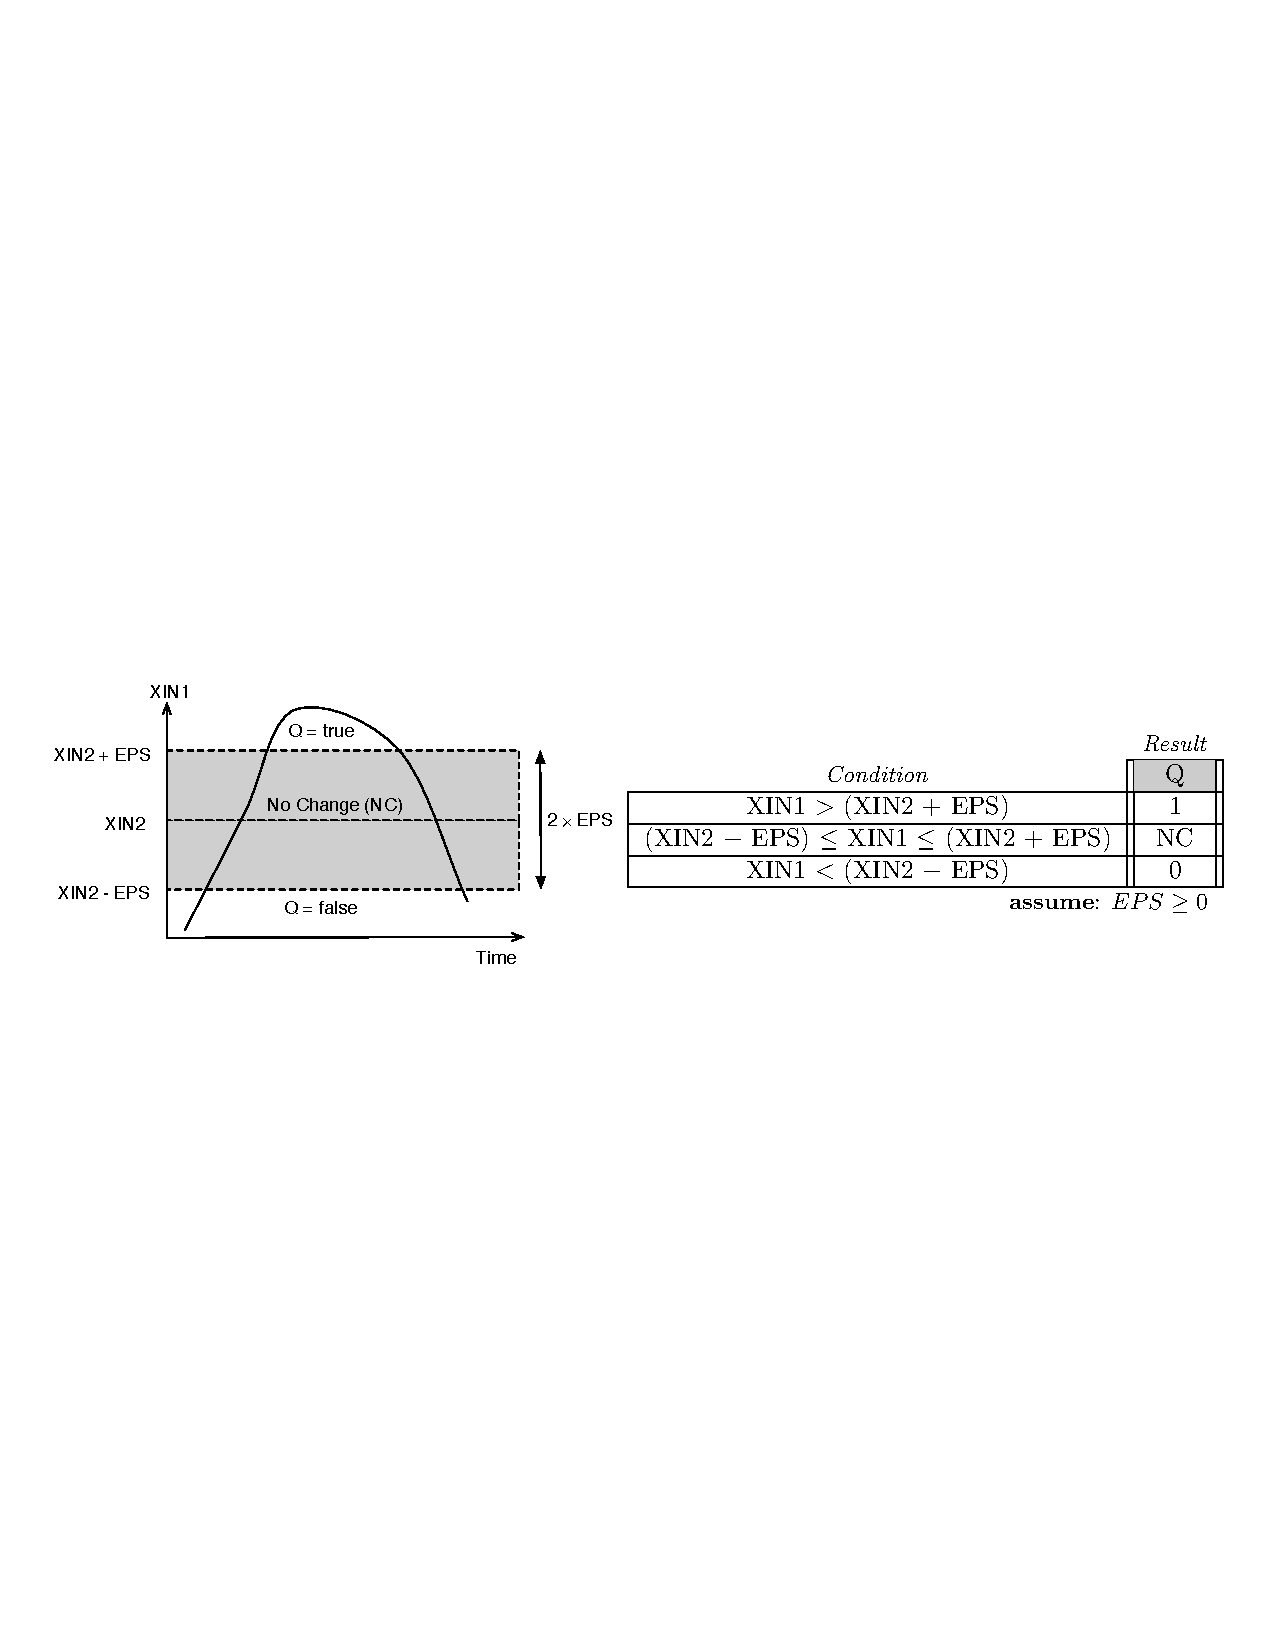
\includegraphics[width=\linewidth]{figures/hysteresis/hysteresis_tab_req}
% \captionof{figure}{\capcolor{Hysteresis: Expected Behaviour \& Tabular Requirement}}
\end{center}\graphspacing

\noindent To prove that the ST implementation of \var{HYSTERESIS}, supplied by IEC~61131-3, satisfies its tabular requirements, we formalize it in PVS:

% HYSTERESIS: ST implementation in pvs
\begin{center}\graphspacing
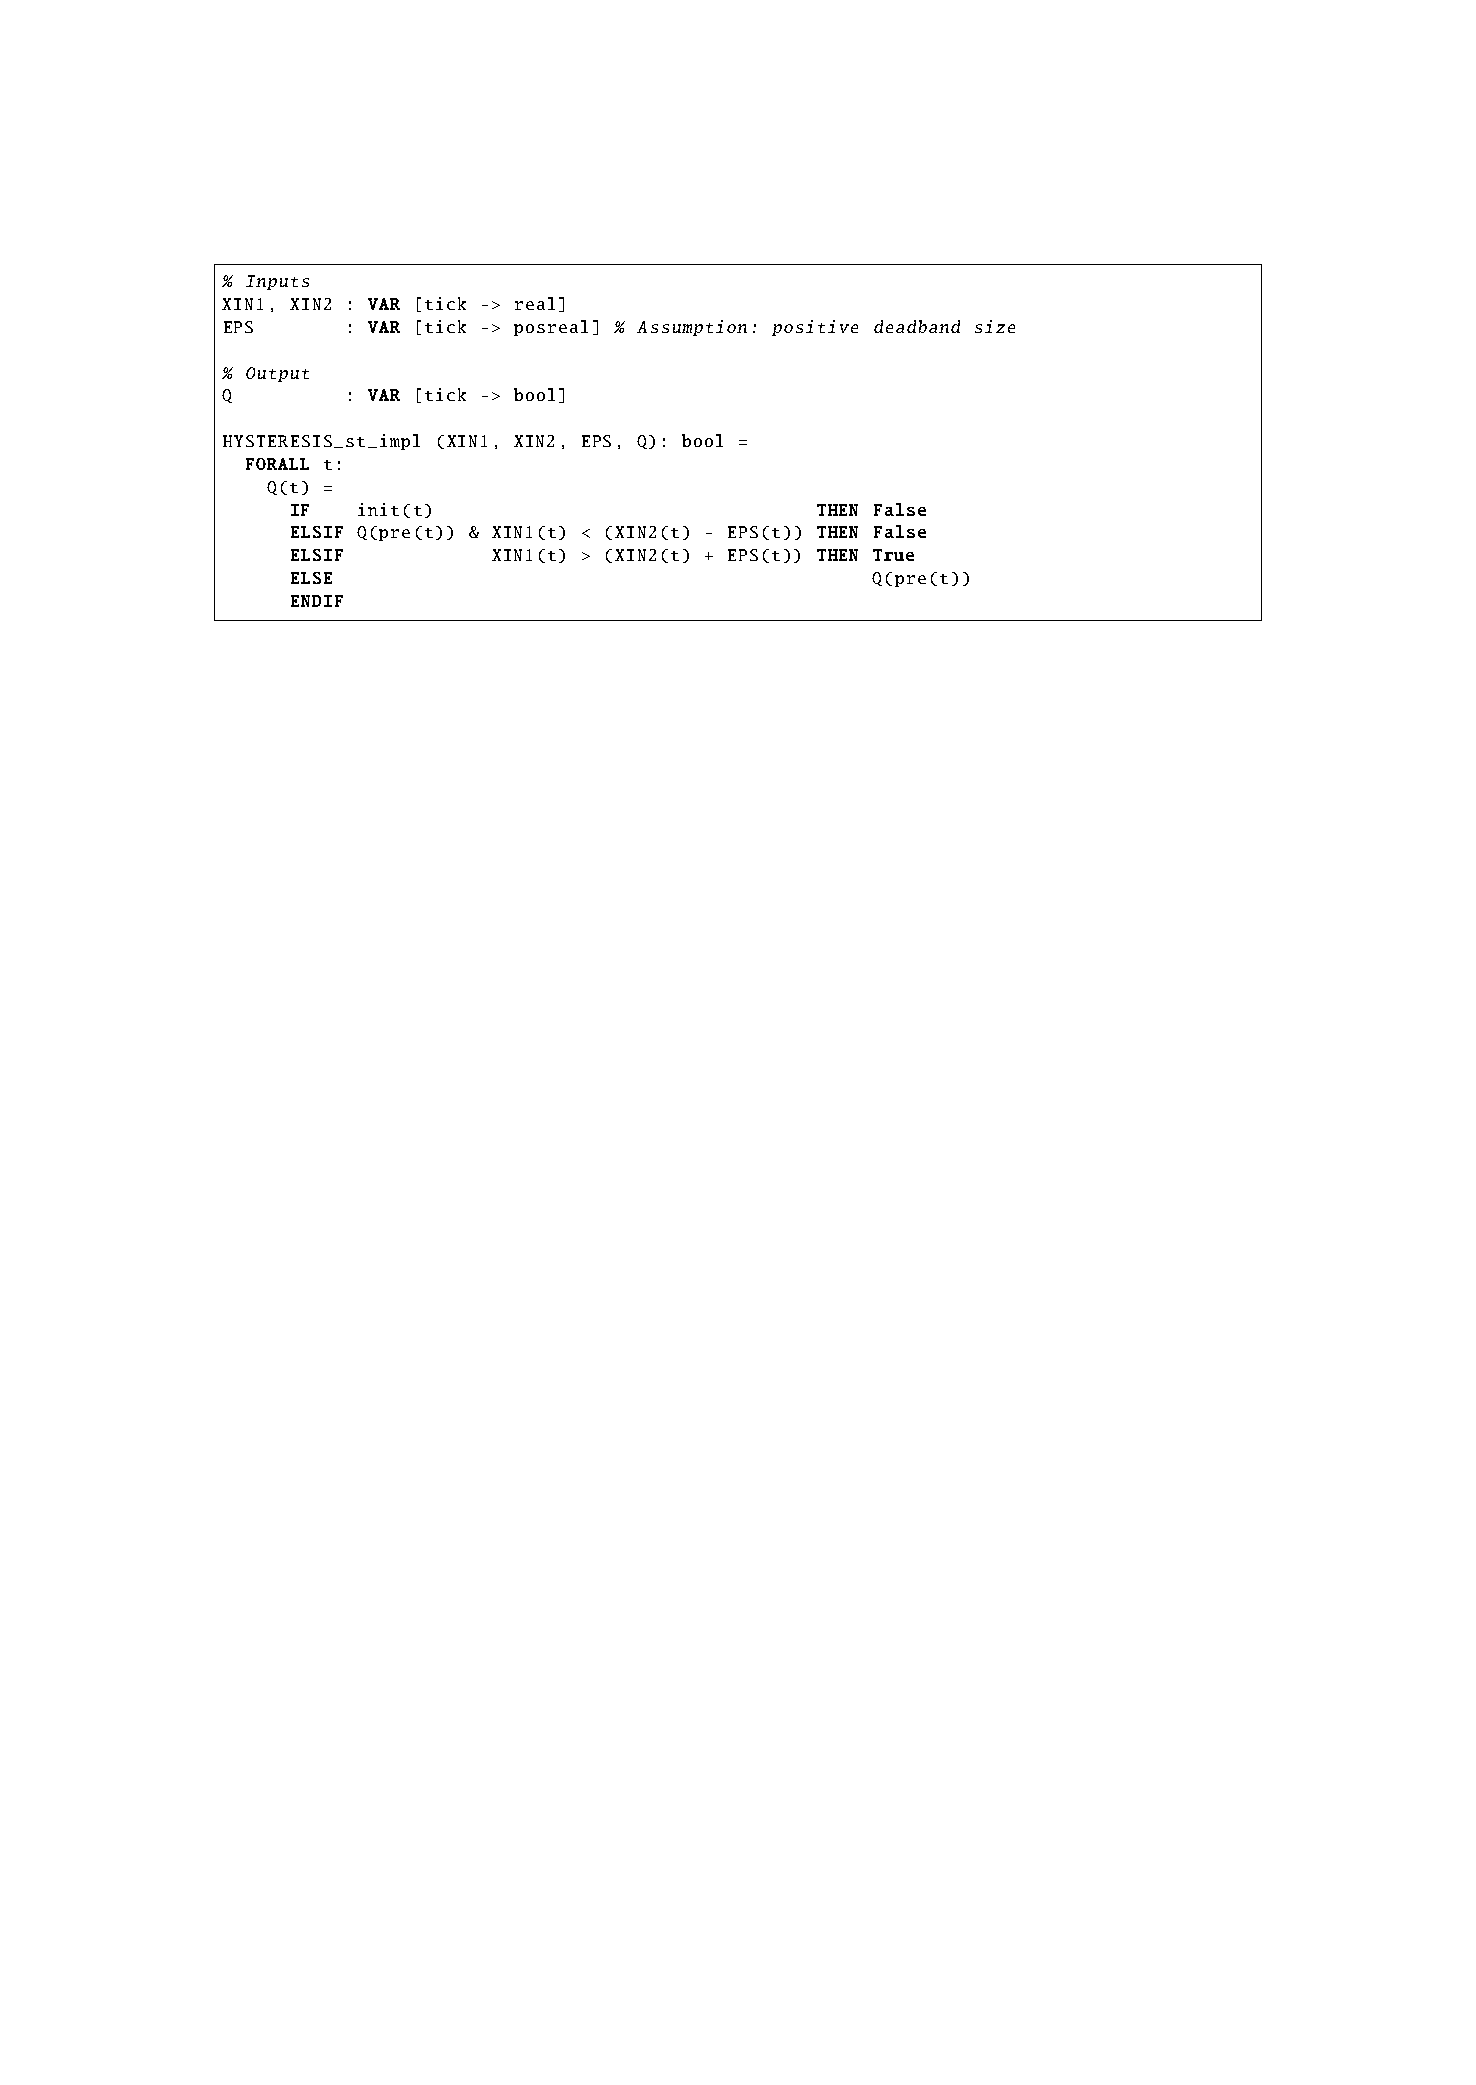
\includegraphics[width=\linewidth]{figures/hysteresis/hysteresis_pvs_st_impl}
% \captionof{figure}{\capcolor{Hysteresis: ST Implementation in PVS}}
\end{center}\graphspacing

\noindent We also translate the tabular requirement of \var{HYSTERESIS} into PVS:

% HYSTERESIS: tabular requirement in pvs
\begin{center}\graphspacing
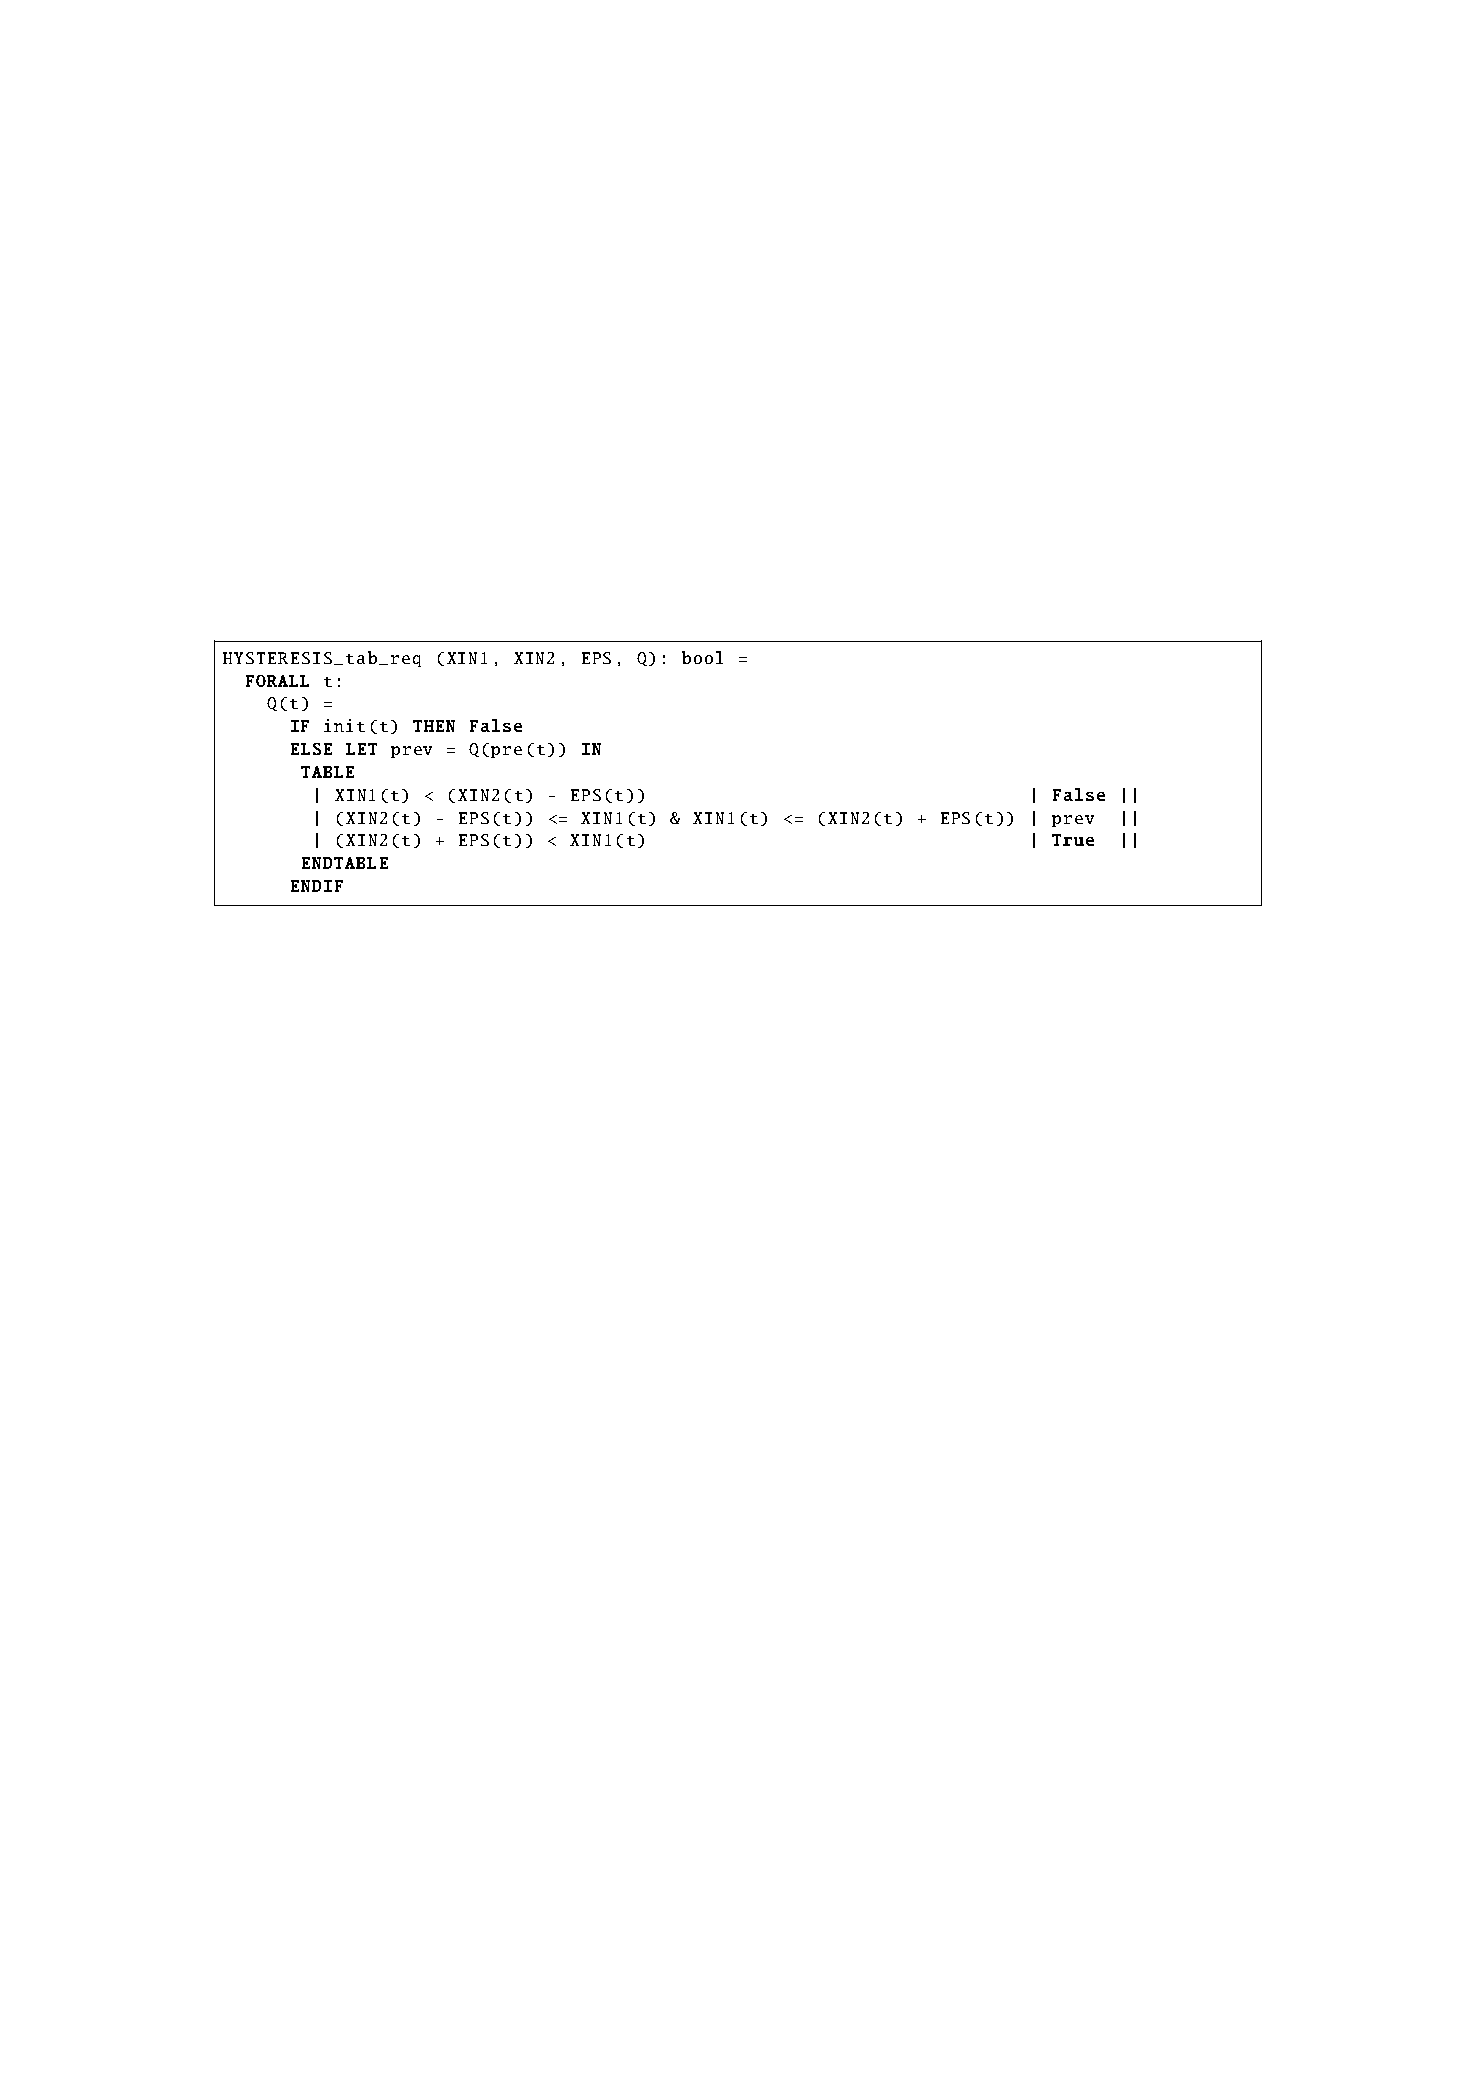
\includegraphics[width=\linewidth]{figures/hysteresis/hysteresis_pvs_tab_req}
% \captionof{figure}{\capcolor{Hysteresis: Tabular Requirement in PVS}}
\end{center}\graphspacing

\noindent Finally, we prove that the ST implementation is:
\begin{itemize}
\item {\color{BrickRed} \emph{correct}} (i.e..,~satisfies its requirement)
\item {\color{BrickRed} \emph{consistent}} (i.e.,~each input vector has a corresponding output)
\end{itemize}

% HYSTERESIS: proofs of correctness and consistency in pvs
\begin{center}\graphspacing
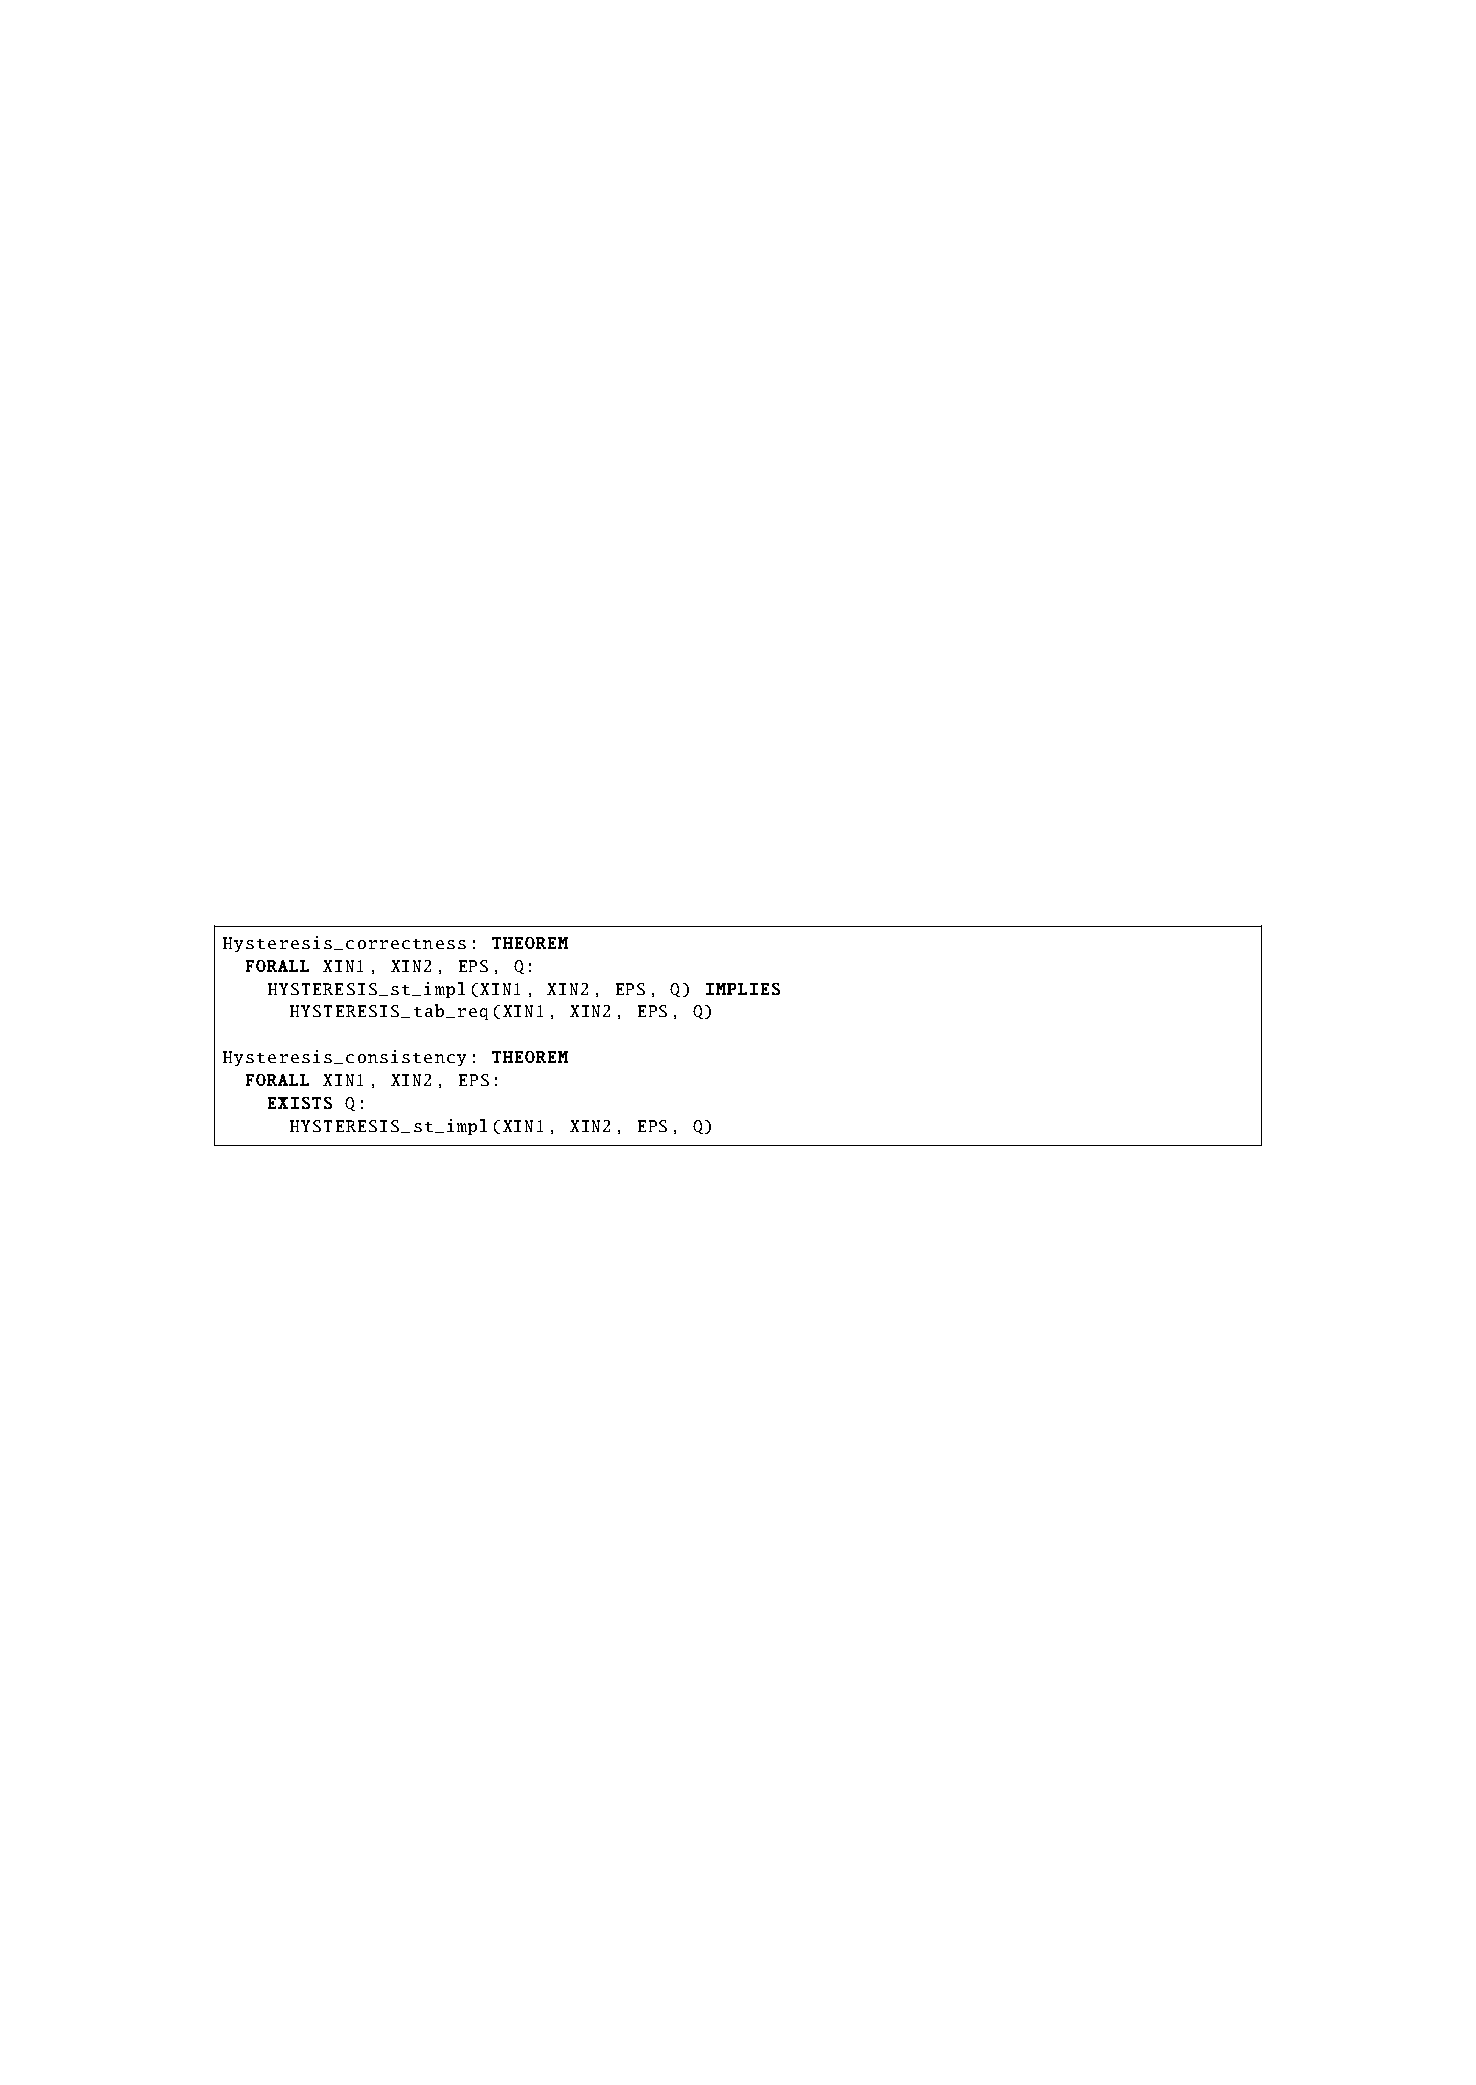
\includegraphics[width=\linewidth]{figures/hysteresis/hysteresis_pvs_theorems}
% \captionof{figure}{\color{Red} Hysteresis: Correctness and Consistency Theorems in PVS}
\end{center}\graphspacing

\noindent \textbf{Remark}. Upon certifying the \var{HYSTERESIS} block, we may reuse its requirements predicate \var{HYSTERESIS\_tab\_req} to certify others (e.g., the \var{LIMITS\_ALARM} block) that use it as a component. 

%%%%%%%%%%%%%%%%%%%%%%%%%%%%%%%%%%%%%%%%%%%%%%%%%%%%%%%%%%%%%%%%%%%%%%%%%%%%%%%%%%%%%%%%%%%%%%%%%%
%%%%%%%%%%%%%%%%%%%%%%%%%%%%%%%%%%%%% Limits Alarm %%%%%%%%%%%%%%%%%%%%%%%%%%%%%%%%%%%%%%%%%%%%%%%
%%%%%%%%%%%%%%%%%%%%%%%%%%%%%%%%%%%%%%%%%%%%%%%%%%%%%%%%%%%%%%%%%%%%%%%%%%%%%%%%%%%%%%%%%%%%%%%%%%

{\color{Blue} \subsection*{Example of Composite FBs: Limits Alarm}}

\noindent Based on the input-output declaration and FBD implementation, as suppled by IEC~61131-3~\cite{IEC:2003:IEP}:

% LIMITS_ALARM: declaration and FBD implementation
\begin{center}\graphspacing
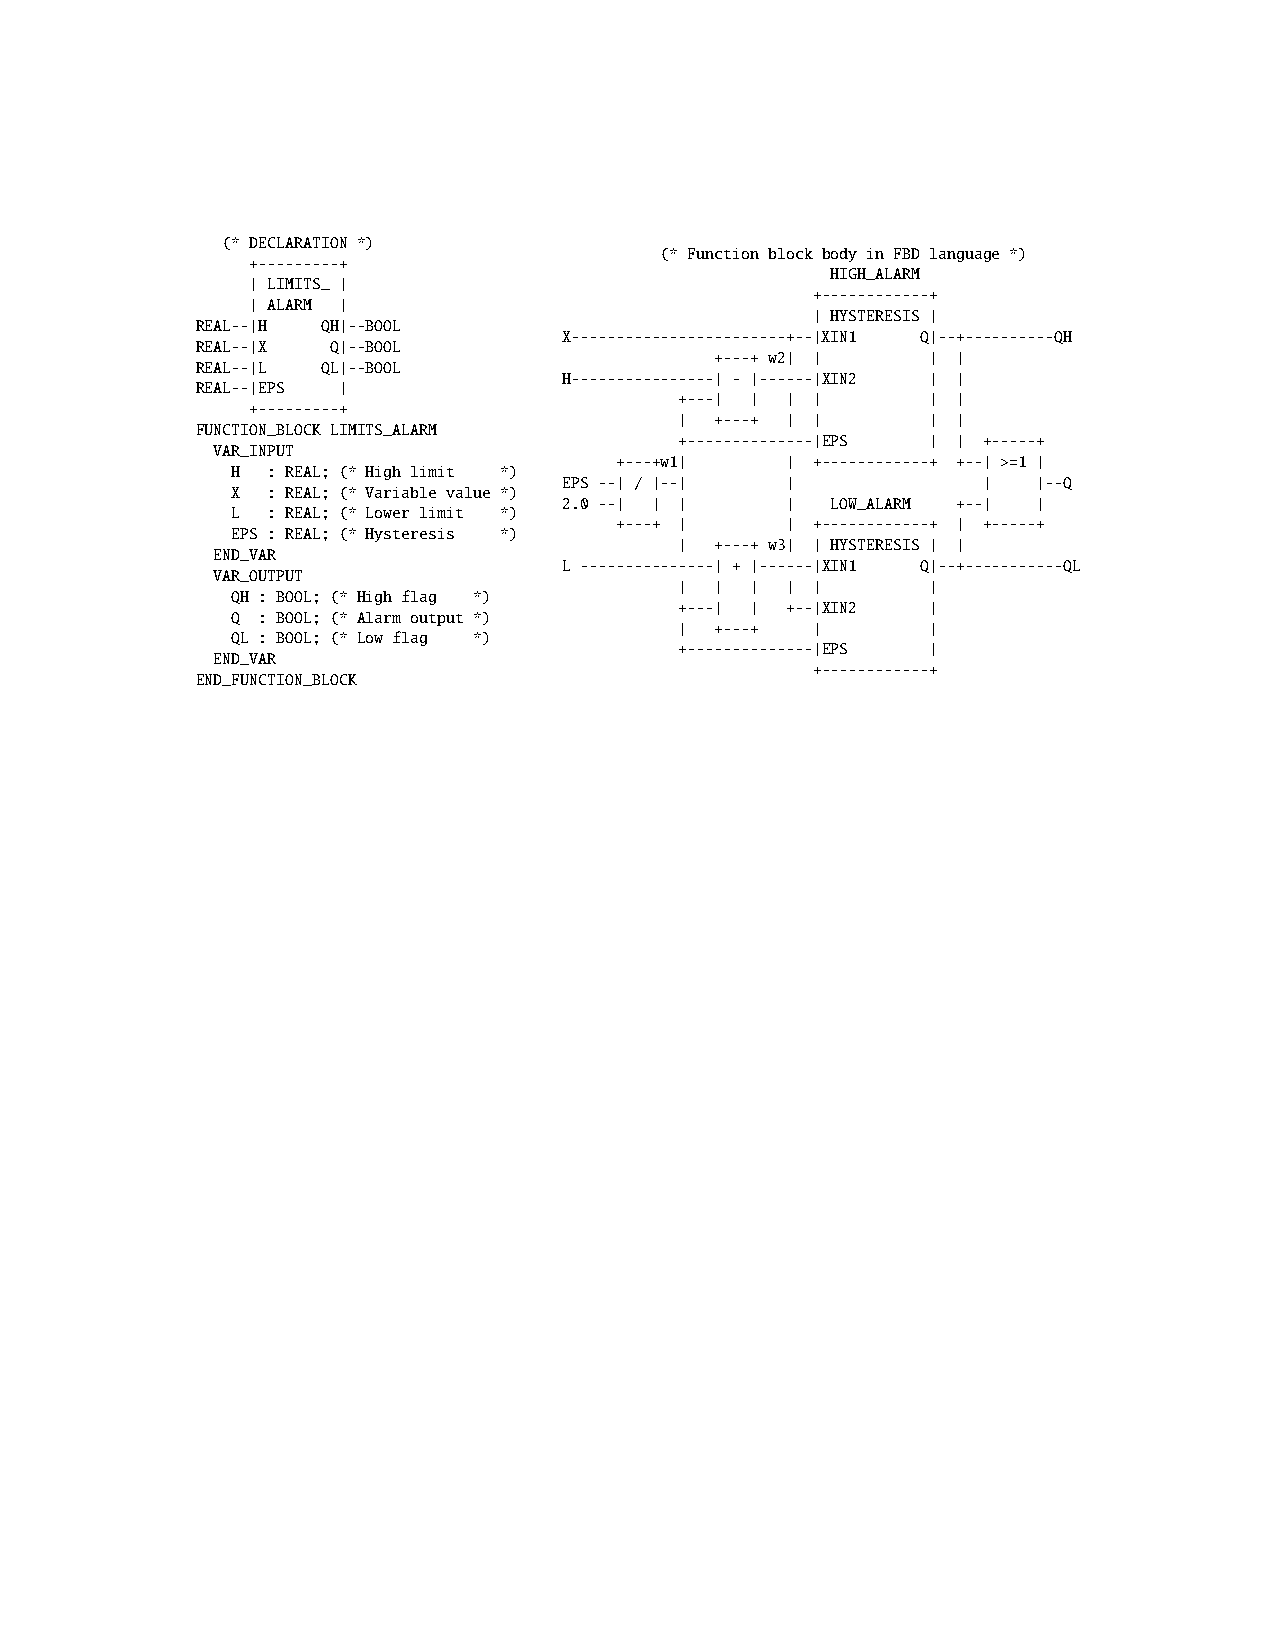
\includegraphics[width=\linewidth]{figures/limits_alarm/limits_alarm_decl}
% \captionof{figure}{\capcolor{Limits Alarm: Declaration and FBD Implementation~\cite{IEC:2003:IEP}}}
\end{center}\graphspacing

\noindent We derive the tabular requirement for \var{LIMITS\_ALARM}:

% LIMITS_ALARM: expected behaviour in tabular expression 
\begin{center}\graphspacing
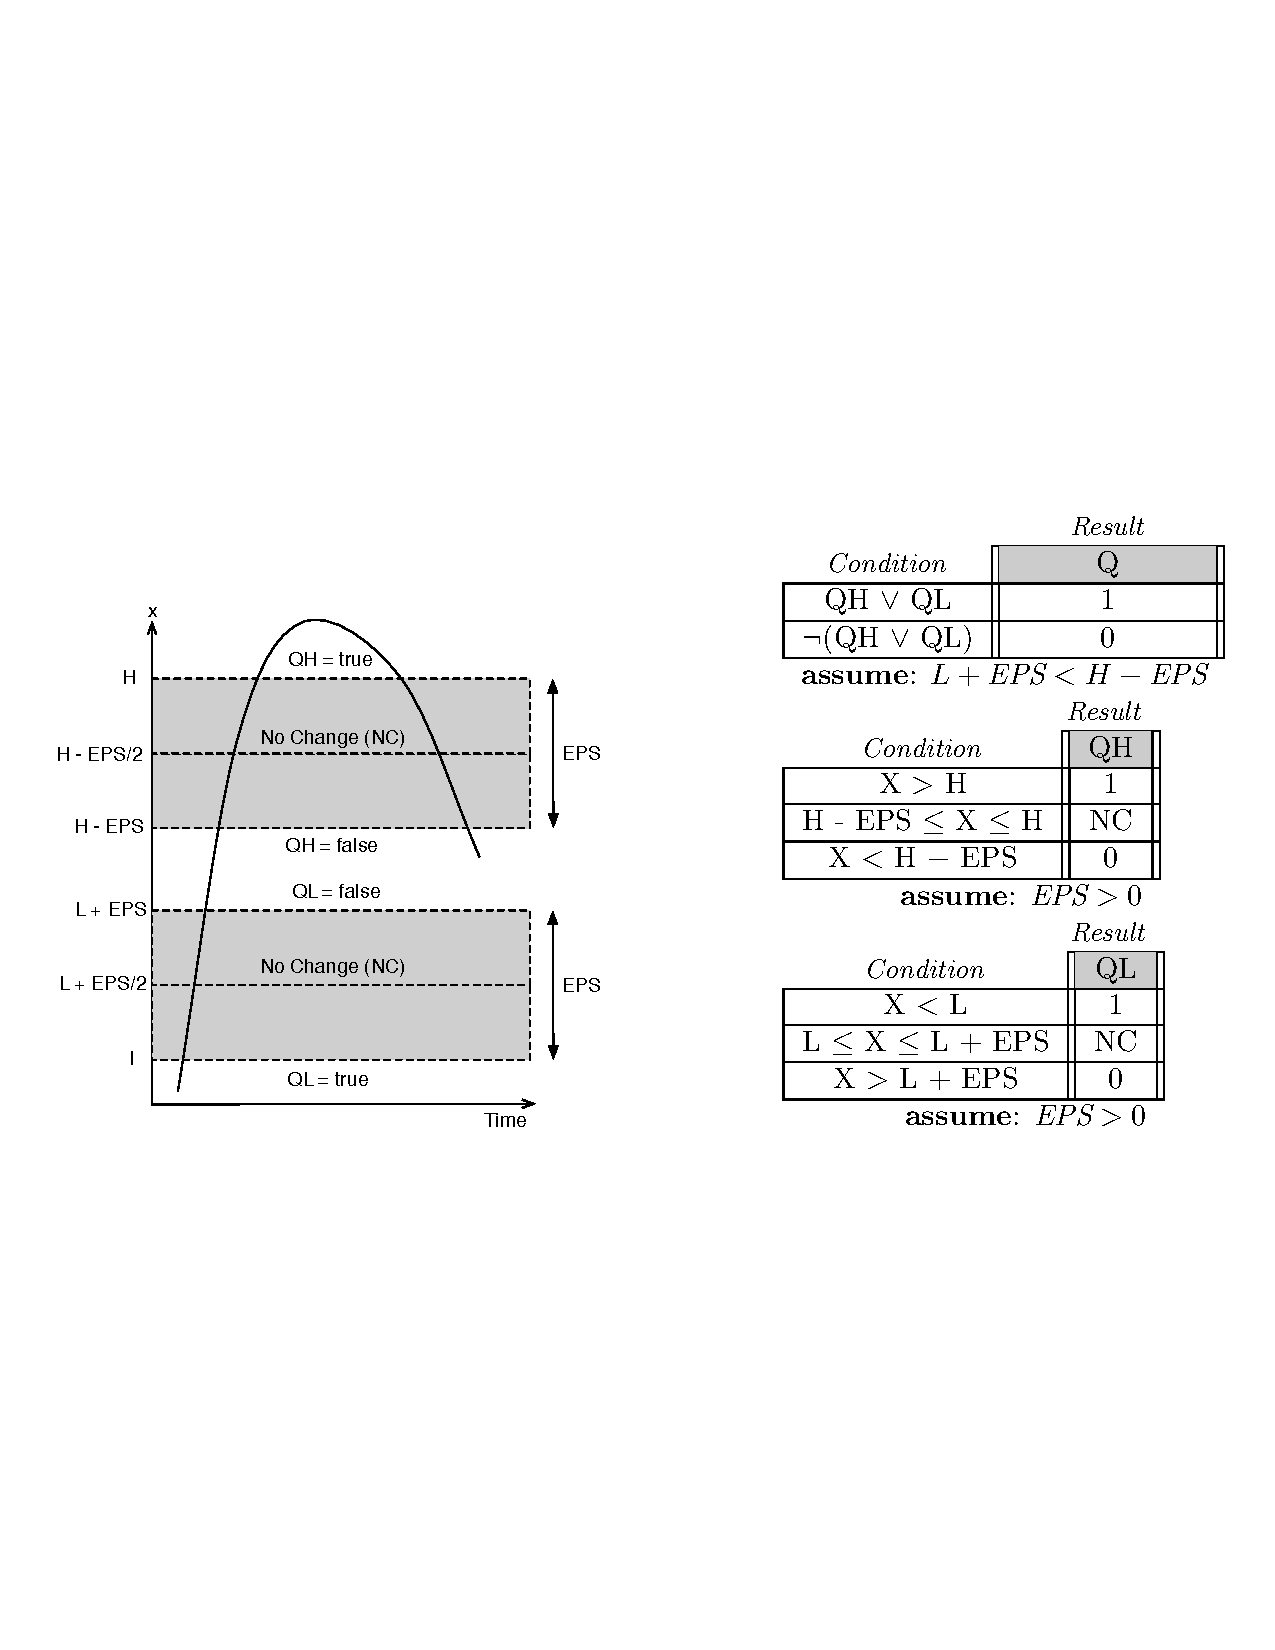
\includegraphics[width=\linewidth]{figures/limits_alarm/limits_alarm_tab_req}
% \captionof{figure}{\capcolor{Limits Alarm: Expected Behaviour \& Tabular Requirements}}
\end{center}\graphspacing

\noindent We formalize the FBD implementation of \var{LIMITS\_ALARM} and its tabular requirements in PVS:

% LIMITS_ALARM: FBD implementation in pvs
\begin{center}\graphspacing
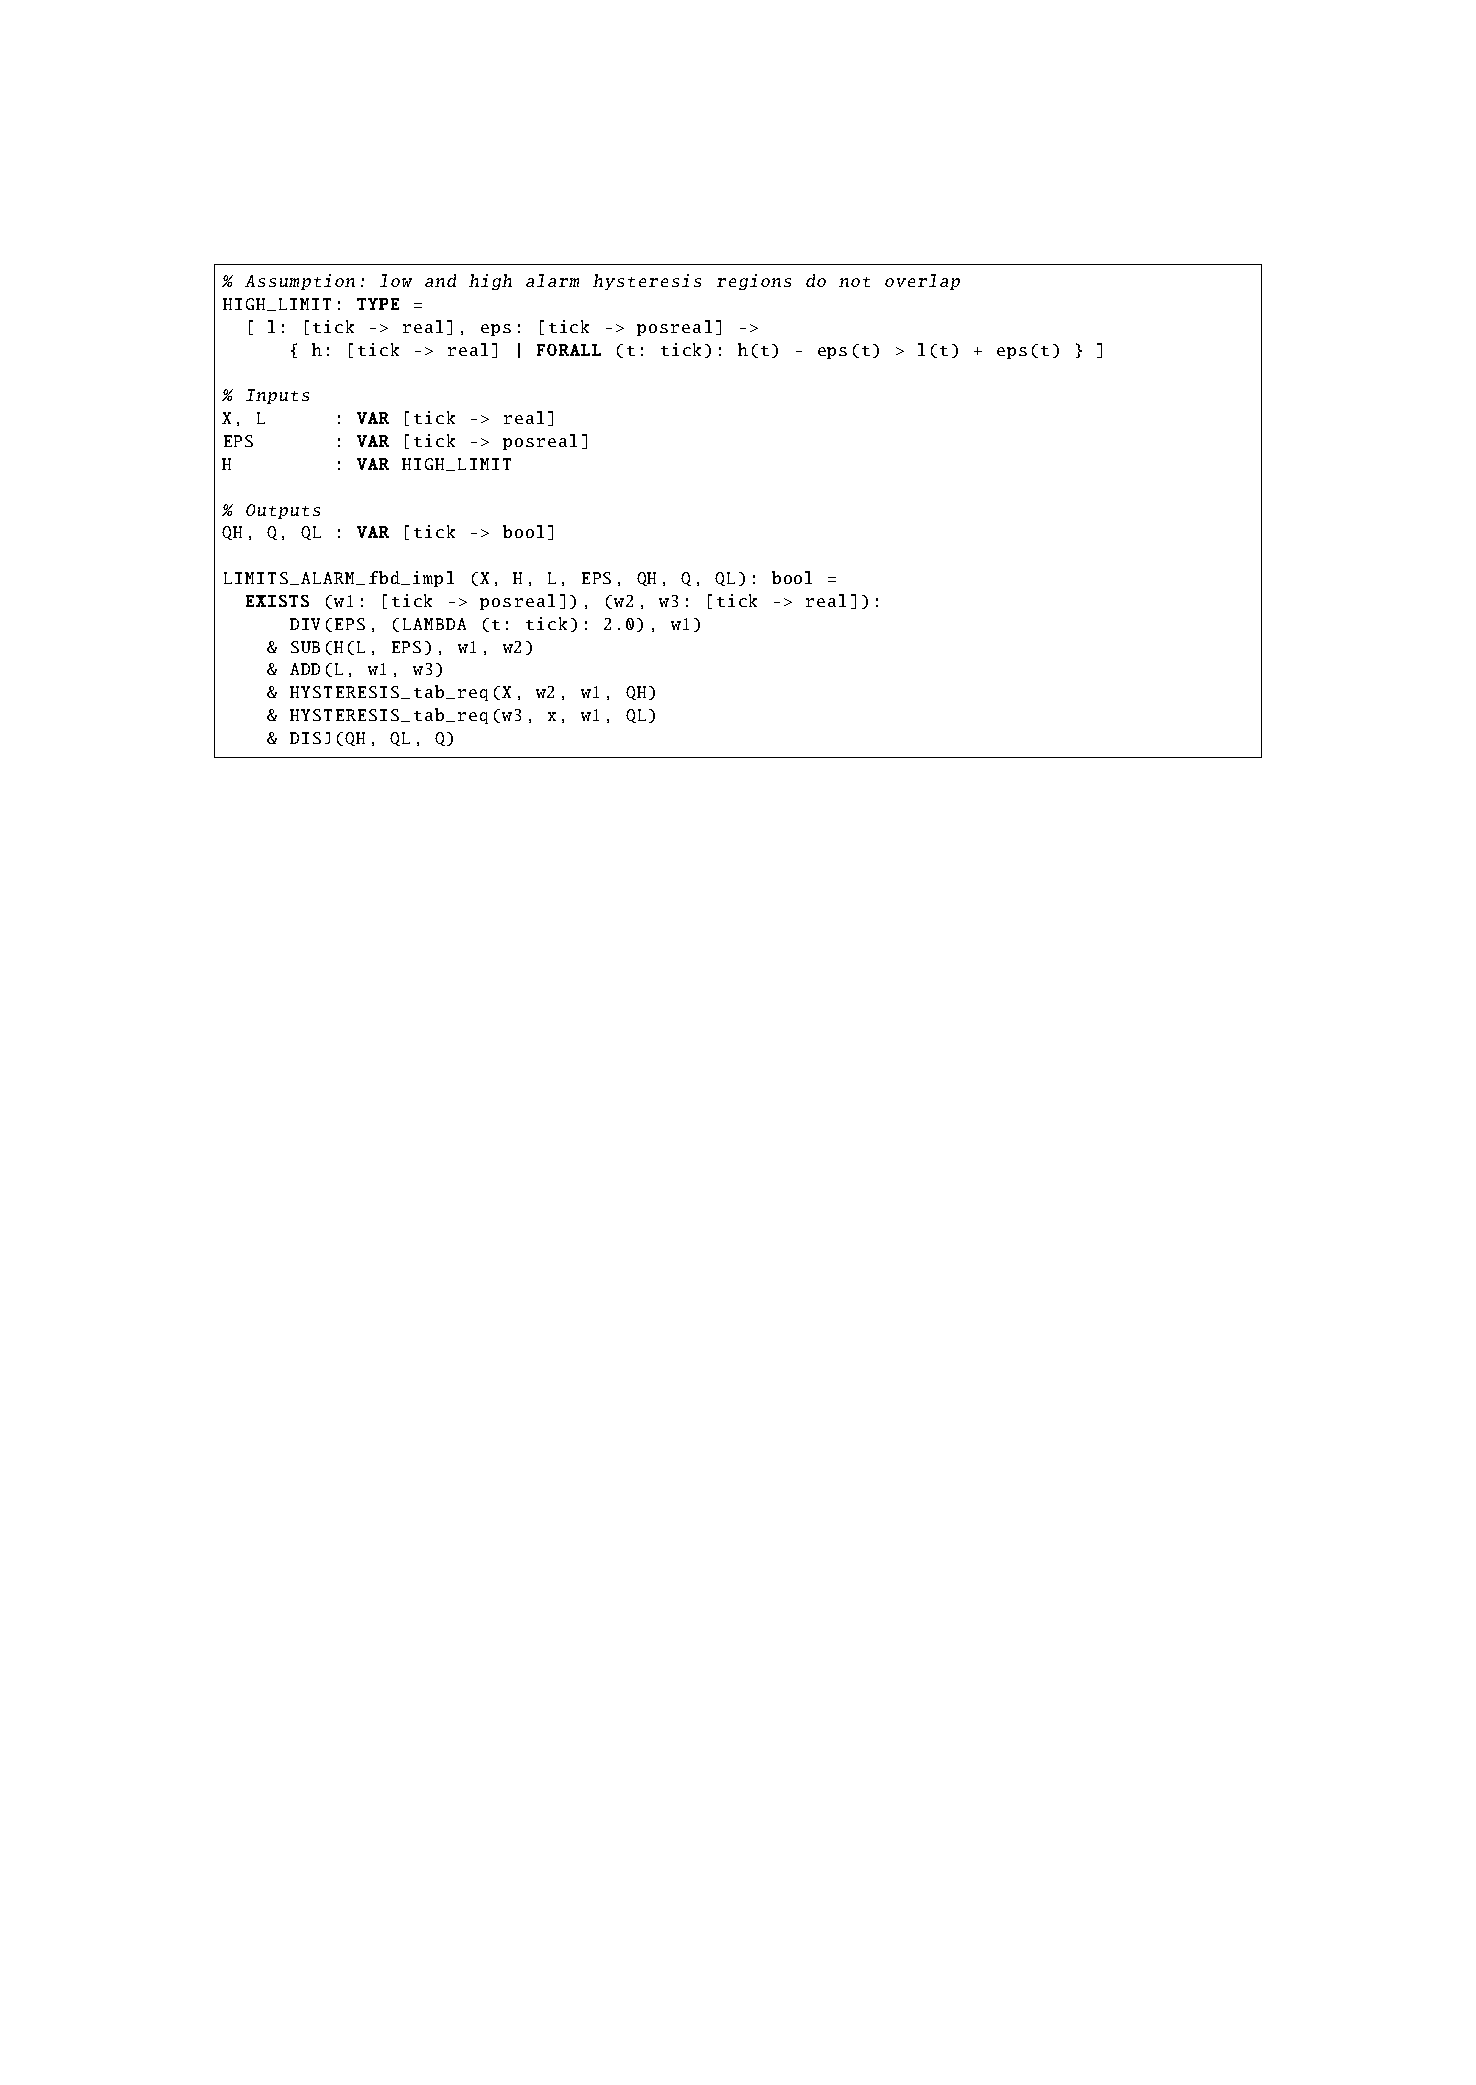
\includegraphics[width=\linewidth]{figures/limits_alarm/limits_alarm_pvs_fbd_impl}
% \captionof{figure}{\capcolor{Limits Alarm: FBD Implementation in PVS}}
\end{center}\graphspacing

\noindent Finally, we prove that the FBD implementation of \var{LIMITS\_ALARM} is {\color{BrickRed} \emph{correct}} and {\color{BrickRed} \emph{consistent}}.

% LIMITS_ALARM: correctness and consistency 
\begin{center}\graphspacing
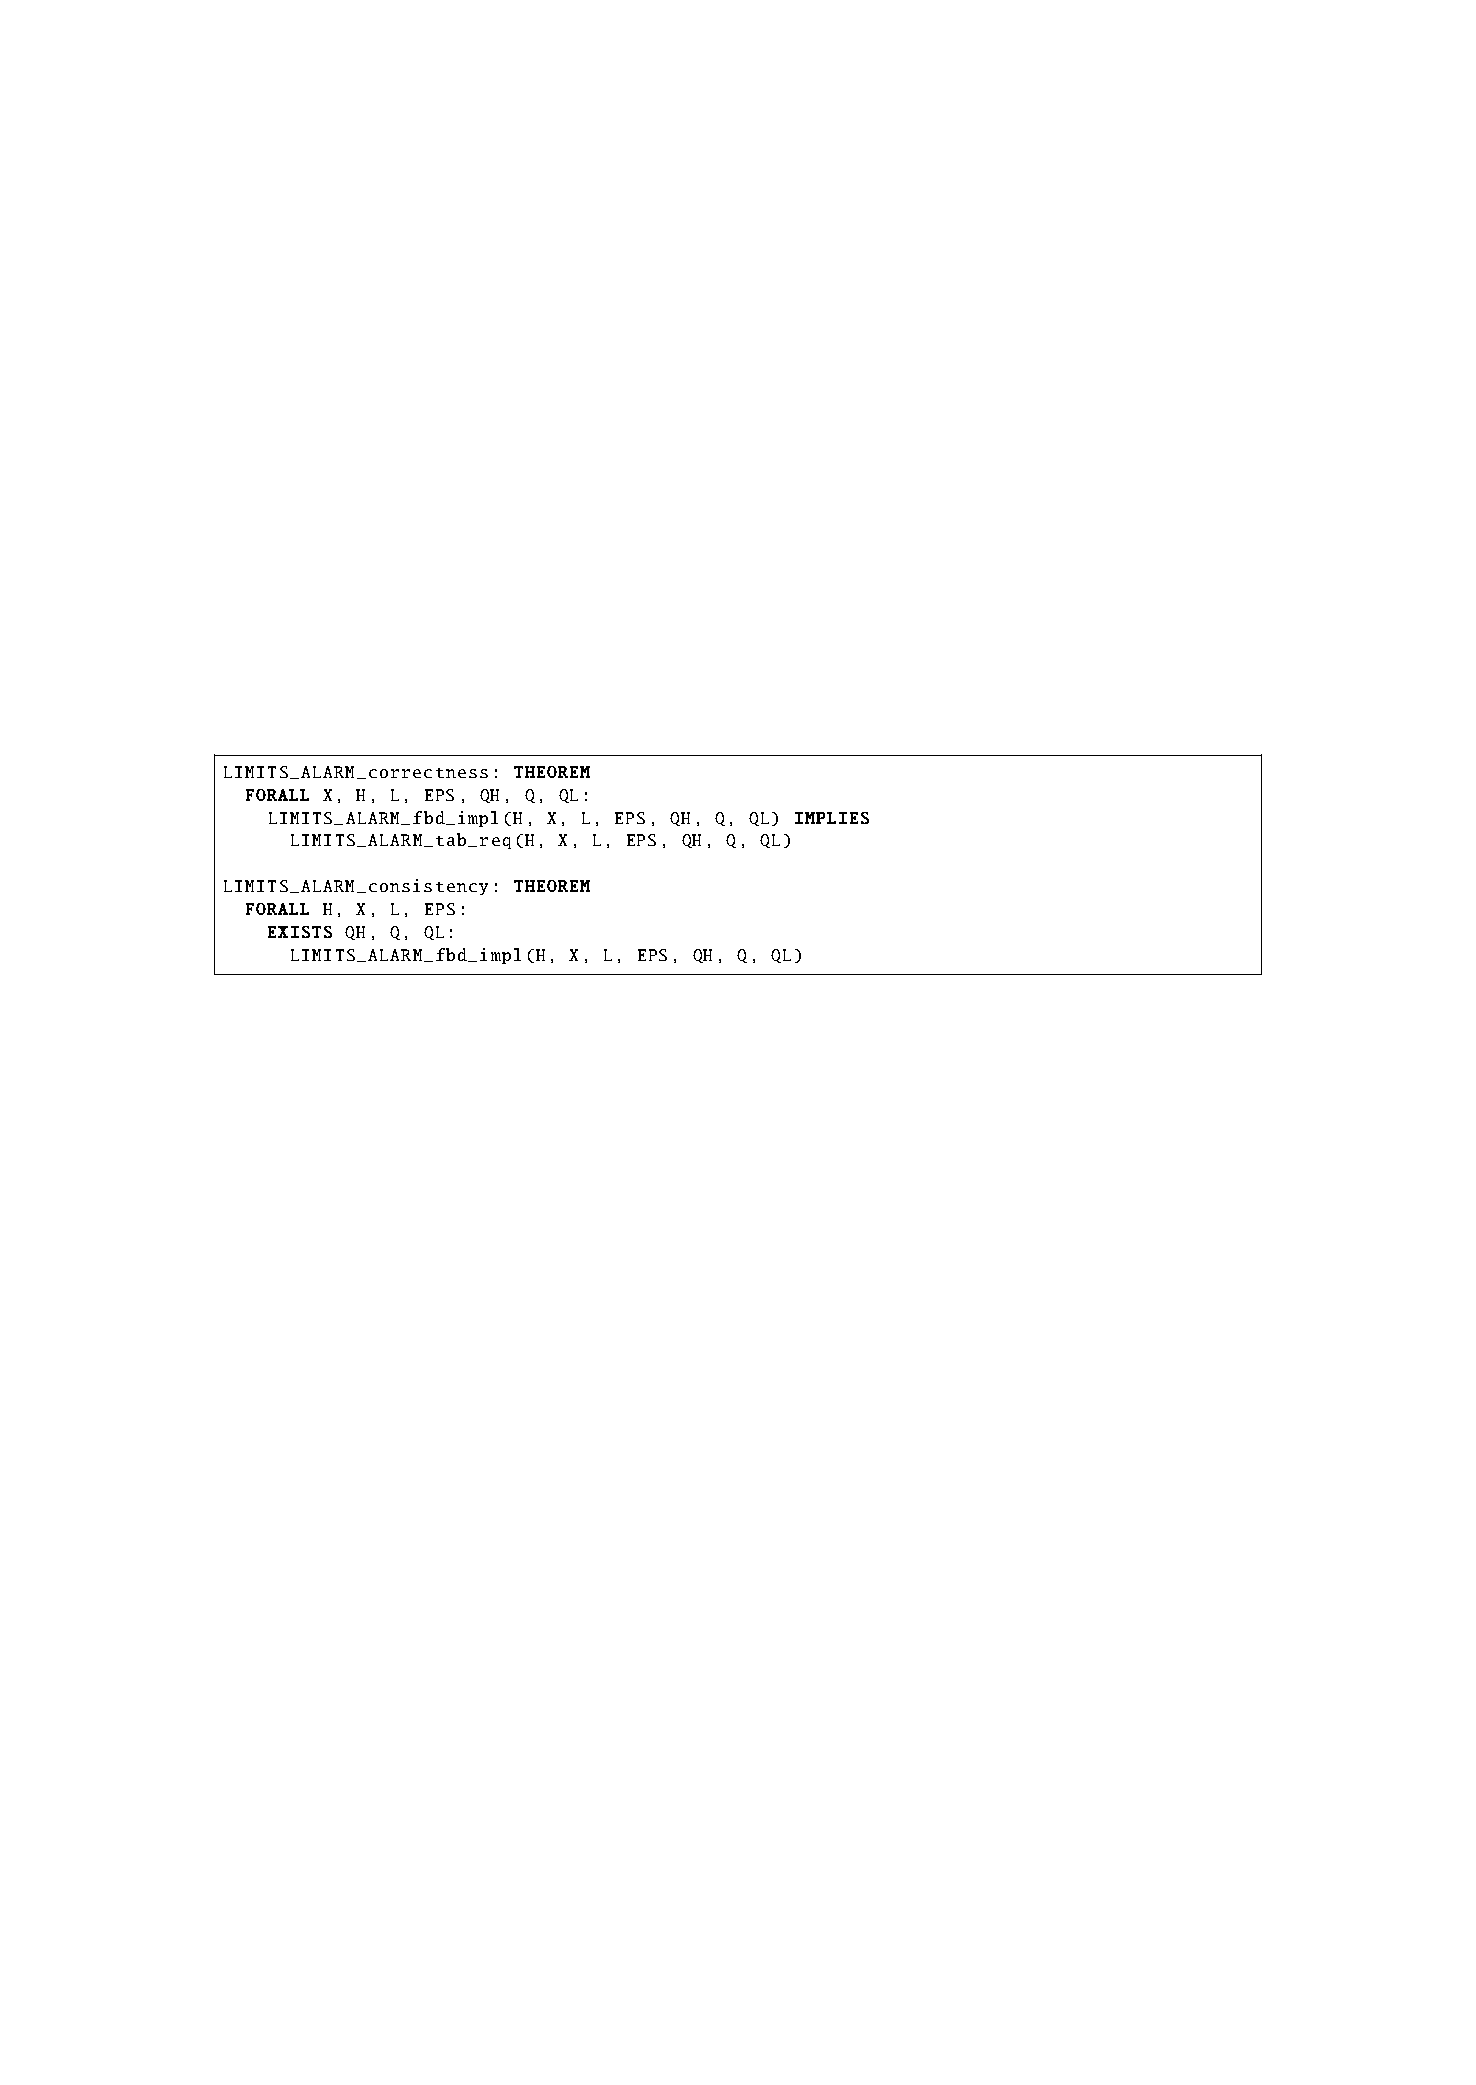
\includegraphics[width=\linewidth]{figures/limits_alarm/limits_alarm_pvs_theorems}
% \captionof{figure}{\color{Red} Limits Alarm: Correctness and Consistency Theorems in PVS}
\end{center}\graphspacing

%%%%%%%%%%%%%%%%%%%%%%%%%%%%%%%%%%%%%%%%%%%%%%%%%%%%%%%%%%%%%%%%%%%%%%%%%%%%%%%%%%%%%%%%%%%%%%%%%%
%%%%%%%%%%%%%%%%%%%%%%%%%%%%%%%%%%%%% Future Work %%%%%%%%%%%%%%%%%%%%%%%%%%%%%%%%%%%%%%%%%%%%%%%%
%%%%%%%%%%%%%%%%%%%%%%%%%%%%%%%%%%%%%%%%%%%%%%%%%%%%%%%%%%%%%%%%%%%%%%%%%%%%%%%%%%%%%%%%%%%%%%%%%%

{\color{Blue} \subsection*{Forthcoming Research}}

\noindent Verification of the TCDD (Trip Computer Design Description) of one of the shutdown systems (SDSs), owned by Ontario Power Generation (OPG), using the pre-verified FBs in IEC~61131-3

%%%%%%%%%%%%%%%%%%%%%%%%%%%%%%%%%%%%%%%%%%%%%%%%%%%%%%%%%%%%%%%%%%%%%%%%%%%%%%%%%%%%%%%%%%%%%%%%%%
%%%%%%%%%%%%%%%%%%%%%%%%%%%%%%%%%%%%% References %%%%%%%%%%%%%%%%%%%%%%%%%%%%%%%%%%%%%%%%%%%%%%%%%
%%%%%%%%%%%%%%%%%%%%%%%%%%%%%%%%%%%%%%%%%%%%%%%%%%%%%%%%%%%%%%%%%%%%%%%%%%%%%%%%%%%%%%%%%%%%%%%%%%

\nocite{*} % Print all references regardless of whether they were cited in the poster or not
\renewcommand{\refname}{{\normalsize \color{Blue} References}}
{\small
\bibliographystyle{plain}
\bibliography{fbs_poster_refs}} 

\end{multicols}
\end{document}